\documentclass{article}

\usepackage[final]{neurips_2019}

\usepackage{xeCJK}
\setCJKmainfont{Noto Sans CJK TC}

\usepackage[
    colorlinks=true,
    urlcolor=blue,
]{hyperref}
\usepackage{url}
\usepackage{booktabs}
\usepackage{amsfonts}
\usepackage{nicefrac}
\usepackage{microtype}
\usepackage{graphicx}
\usepackage{xcolor}
\usepackage{lipsum}


\newcommand{\note}[1]{\textcolor{blue}{{#1}}}

\title{
  NTU 2025 Fall Applied Deep Learning HW2 Report \\
  \vspace{1em}
  \small{\normalfont NTU CSIE 5431 Applied Deep Learning}
}

\author{
  CHIH-HAO LIAO \\
  {\hypersetup{urlcolor=black}\href{https://www.fo.ntu.edu.tw/}{School of Forestry and Resource Conservation}}\\
  {\hypersetup{urlcolor=black}\href{https://www.bebi.ntu.edu.tw/}{Graduate Institute of Biomedical Electronics and Bioinformatics}}\\
  {\hypersetup{urlcolor=black}\href{https://www.ntu.edu.tw/}{National Taiwan University}}\\
  {\hypersetup{urlcolor=black}\href{mailto:R11625015@ntu.edu.tw}{\texttt{R11625015@ntu.edu.tw}}} \\
}

\begin{document}

\maketitle

\section{Q1: LLM Tuning (10\%)}
\subsection{Describe: (6\%)}
\begin{itemize}
    \item How much training data did you use? (2\%)
    \item How did you tune your model? (2\%)
    \item What hyper-parameters did you use? (2\%)
\end{itemize}

\textbf{How much training data did you use?}

The training employed $10,000$ examples from the dataset provided by TA. Each example consists of an instruction field, which contains a sentence in either modern or classical Chinese accompanied by a translation prompt, and an output field, which provides the corresponding translation in the target language. This dataset thus facilitates bidirectional translation between modern and classical Chinese.

\textbf{How did you tune your model?}

The model was fine-tuned using LoRA (Low-Rank Adaptation) \citep{hu2022lora} in combination with 4-bit quantization via the BitsAndBytes library, enabling efficient parameter-efficient tuning of the base model \href{https://huggingface.co/Qwen/Qwen3-4B}{Qwen/Qwen3-4B} \citep{qwen3technicalreport}. LoRA adapters were applied to all linear layers of the model, allowing fine-tuning with a significantly reduced number of trainable parameters while preserving overall model performance \citep{dettmers2023qlora}.

The key training configurations included:

\begin{itemize}
    \item 4-bit quantization to reduce memory consumption and enable training on limited GPU resources.
    \item BFloat16 mixed precision training to improve computational efficiency.
    \item Gradient checkpointing to lower memory usage during backpropagation.
    \item Cosine learning rate scheduler with a 3\% warmup ratio to stabilize training.
    \item Per-device batch size of 2 with gradient accumulation over 8 steps to simulate a larger effective batch size.
    \item Evaluation every 100 steps to monitor performance during training.
\end{itemize}

\textbf{What hyper-parameters did you use?}

The key hyperparameters used in training were listed in Table \ref{tab:hyperparams}.

\begin{table}[h!]
    \centering
    \caption{Training hyper-parameters used for LoRA fine-tuning of Qwen/Qwen3-4B.}
    \begin{tabular}{ l l }
        \hline
        \textbf{Hyper-parameter}    & \textbf{Value}                  \\
        \hline
        Base model                  & Qwen/Qwen3-4B                  \\
        LoRA rank ($r$)             & 64                              \\
        LoRA alpha                  & 64                              \\
        Quantization                & 4-bit                           \\
        Precision                   & BFloat16 mixed precision        \\
        Learning rate               & $2 \times 10^{-5}$              \\
        Learning rate scheduler     & Cosine with 3\% warmup ratio    \\
        Per-device train batch size & 2                               \\
        Per-device eval batch size  & 2                               \\
        Gradient accumulation steps & 8                               \\
        Gradient checkpointing      & Enabled                         \\
        Maximum training steps      & 1000                            \\
        Evaluation strategy         & Steps, every 100 steps          \\
        Checkpoint saving           & Every 100 steps, keep last only \\
        Data loader workers         & 4, pinned memory enabled        \\
        TF32 computation            & Enabled                         \\
        Training enabled            & False                           \\
        Evaluation enabled          & True                            \\
        Overwrite output directory  & Enabled                         \\
        \hline
    \end{tabular}
    \label{tab:hyperparams}
\end{table}


\newpage

\subsection{Show your performance: (4\%)}
\begin{itemize}
    \item What is the final performance of your model on the public testing set? (2\%)
    \item Plot the learning curve on the public testing set (2\%)
\end{itemize}

\textbf{What is the final performance of your model on the public testing set?}
\begin{itemize}
    \item Training loss: 2.377731004714966
    \item Evaluation loss: 6.481075286865234
    \item Mean perplexity: 9.94803125
\end{itemize}

\textbf{Plot the learning curve on the public testing set}
\begin{figure}[h!]
    \centering
    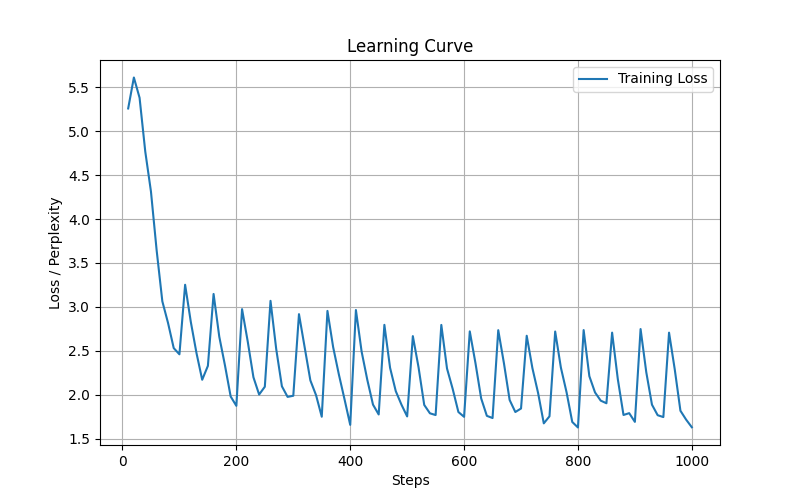
\includegraphics[width=0.7\textwidth]{learning_curve.png}
    \caption{Learning curve showing training and evaluation loss over steps on the public testing set.}
    \label{fig:learning_curve}
\end{figure}

\newpage

\section{Q2: LLM Inference Strategies (5\%)}
\subsection{Zero-Shot (1\%)}
\begin{itemize}
    \item What is your setting? How did you design your prompt? (1\%)
\end{itemize}

\textbf{What is your setting? How did you design your prompt?}

For the zero-shot inference, we use a single instruction to prompt the LLM without providing any examples, which is the same as the QLoRA prompt. The prompt is designed to provide clear context and role for the model:

\begin{itemize}
    \item We instruct the model to act as a top Chinese literature professor and perform classical-modern Chinese translation tasks.
    \item The prompt explicitly asks the model to output the translation result.
\end{itemize}

\textbf{Example Prompt:}

\begin{verbatim}
你是世界頂尖的中文系教授,以下是文言文與白話文轉換的任務。
根據指令要求,生成合適的翻譯。
指令:{instruction}
請輸出翻譯結果:
\end{verbatim}

This ensures that even without examples, the model understands the task and expected output format.

\subsection{Few-Shot (In-context Learning) (2\%)}
\begin{itemize}
    \item What is your setting? How did you design your prompt? (1\%)
    \item How many in-context examples are utilized? How you select them? (1\%)
\end{itemize}

\textbf{What is your setting? How did you design your prompt?}

Few-shot learning provides the model with several in-context examples before the actual instruction. This helps guide the LLM towards the desired style and output format. The prompt is structured as follows:

\begin{itemize}
    \item Two examples are provided: one translating modern Chinese to classical Chinese, and another translating classical Chinese to modern Chinese.
    \item Each example follows an instruction-answer format, making the task clear to the model.
\end{itemize}

\textbf{How many in-context examples are utilized? How you select them?}

\begin{itemize}
    \item We use two in-context examples, carefully selected to cover both translation directions (modern $\leftrightarrow$ classical).
    \item Examples are representative and concise, helping the model generalize the instruction without overwhelming it.
\end{itemize}

\textbf{Example Few-Shot Prompt:}

\begin{verbatim}
指令:翻譯成文言文:
雅裏惱怒地說:從前在福山田獵時,你誣陷獵官,現在又說這種話。
回答:雅裏怒曰:昔畋於福山,卿誣獵官,今復有此言。

指令:翻譯成白話文:
議雖不從,天下咸重其言。
回答:他的建議雖然不被采納,但天下都很敬重他的話。

指令:<user instruction>
回答:<output>
\end{verbatim}

\subsection{Comparison: (1\%)}
\begin{itemize}
    \item What's the difference between the results of zero-shot, few-shot, and LoRA? (2\%)
\end{itemize}

\textbf{What's the difference between the results of zero-shot, few-shot, and LoRA?}
\begin{itemize}
    \item \textbf{Zero-Shot}
    
    Performance depends entirely on the model's pretraining and general reasoning. It works reasonably well for simple or straightforward tasks but may produce inconsistent or stylistically incorrect translations for complex instructions.
    
    \item \textbf{Few-Shot (In-context Learning)}
    
    Providing examples significantly improves output quality. The model better mimics the desired translation style and format, reduces errors, and maintains consistency across translations.

    \item \textbf{LoRA Fine-tuning}
    
    Low-Rank Adaptation (LoRA) further boosts performance by fine-tuning the model on domain-specific datasets. Compared to few-shot prompting, LoRA reduces reliance on in-context examples, ensures more stable translation accuracy, and can generalize better to unseen instructions.
\end{itemize}

\textbf{Summary:}
Zero-shot inference is quick to deploy and highly flexible, but its outputs may lack consistency and stylistic accuracy. Few-shot prompting improves reliability and better aligns the outputs with the desired format, using the model’s existing weights without additional training. LoRA fine-tuning achieves the highest quality and stability, though it demands more computational resources and training time. Overall, the performance hierarchy is: LoRA fine-tuning > Few-shot > Zero-shot, with the trade-off being speed versus output quality.

\section{Q3: Bonus: Try Llama3-Taiwan (8B) (2\%)}
\begin{itemize}
    \item \href{https://huggingface.co/yentinglin/Llama-3.1-Taiwan-8B}{Llama-3-8b} trained by traditional Chinese data
    \item Tune this model on the classical chinese data
    \item Describe your experimental settings and compare the results to those obtained from your original methods
\end{itemize}

Although there was insufficient time to fully train this model, we can provide a brief description of the experimental setup. The configuration is essentially the same as used in the QLoRA experiments, with the only difference being the substitution of the pretrained base model. Regarding the outcomes, while a fully optimized model was not obtained, observations from the base model indicate that Llama-3.1-Taiwan-8B is expected to outperform Qwen/Qwen3-4B, as it has been specifically pretrained on traditional Chinese datasets.

\bibliographystyle{unsrt}
\bibliography{references}

\end{document}
